% Student template

\clearpage
\newpage
\mbox{~}
\clearpage
\newpage
\unskip

\checkoddpage

% Returns a default file if not found
\providecommand\dfincludegraphics[2][]{
	\IfFileExists{#2}
	{
		\includegraphics[#1]{#2}
	}
	{
		%\fbox{File not found}
	}
}

\providecommand\studentbackground[2]{
	\sectionmark{Steckbrief - \stdname}

	% Ring
	\def\ringx{20pt}
	\def\ringy{250pt}
	\def\ringwidth{250pt}
	\def\ringimgwidth{180pt}
	\def\ringoffset{(\ringwidth - \ringimgwidth) / 2}
	\ifoddpage
		\def\ringx{-\paperwidth - 325pt} % ringwidth + 2 * ringx % Nope, idk anymore
	\else\fi

	% Frame and QR-Code
	\def\framex{160pt}
	\def\framey{20pt}
	\def\framewidth{180pt}
	\def\frameimgwidth{160pt}
	\def\frameoffset{(\framewidth - \frameimgwidth) / 2}
	\def\qrcodex{90pt}
	\ifoddpage
		\def\framex{540pt} % paperwidth - framewidth / 2 % Nope, idk anymore
		\def\qrcodex{470pt}
	\else\fi

	\AddToShipoutPictureBG*{
		\AtTextUpperLeft{
			\put(-\ringx + \ringoffset, -\ringy + \ringoffset){
				\def\imgpath{parts/generated/students/figures/36_#1.jpg}
				\IfFileExists{\imgpath}{}
				{
					\def\imgpath{bloed.png}
				}
				\includegraphics[keepaspectratio=true, width=\frameimgwidth]{\imgpath}
			}
			\put(-\ringx, -\ringy){
				
\includegraphics[keepaspectratio=true, width=\ringwidth]{ring.png}
			}
		}
		\AtTextLowerLeft{
			\put(\textwidth - \framex + \frameoffset, \framey + \frameoffset + 8pt){
				\def\imgpath{parts/generated/students/figures/11_#1.jpg}
				\IfFileExists{\imgpath}{}{
					\def\imgpath{enkel.png}
				}
				\includegraphics[keepaspectratio=true, width=\frameimgwidth]{\imgpath}
			}
			\put(\textwidth - \framex, \framey){
				\evenflip[keepaspectratio=true, width=\framewidth]{rahmen.png}
			}
			\put(\textwidth - \qrcodex, \framey - 25pt){
				\def\stdqrcode{#2}
				\ifdefempty{\stdqrcode}{}{
					\qrcode[nolink, height=0.7in]{#2}
				}
			}
			\put(\textwidth - \qrcodex, 250pt){
				\evenflip[keepaspectratio=true, height=3cm]{captain.png}
			}
		}
	}
}

\providecommand\studentinit{
	% Steckbrief Tabelle
	\ifoddpage
		\def\tablex{-0cm}
		\def\tablewidth{0.55\linewidth} % Right side
	\else
		\def\tablex{0.5\linewidth}
		\def\tablewidth{0.55\linewidth} % Left side
	\fi

	\hspace*{\tablex}\vspace*{1.4cm}\begin{minipage}{\tablewidth}
		\vspace*{.5cm}
		\begin{normalsize}
			\begin{tabular}{@{}ll@{}}
				\textbf{Name:}          & \stdname                                                  \\
				\textbf{Geburtstag:}    & \multicolumn{1}{p{\tablewidth}}{\RaggedRight\stdbirthday} \\
				\textbf{Lieblingsfach:} & \multicolumn{1}{p{\tablewidth}}{\RaggedRight\stdfavsub}   \\
				\textbf{Hassfach:}      & \multicolumn{1}{p{\tablewidth}}{\RaggedRight\stdhatesub}  \\
				\textbf{Hobbies:}       & \multicolumn{1}{p{\tablewidth}}{\RaggedRight\stdhobbies}  \\
				\textbf{Musik:}         & \multicolumn{1}{p{\tablewidth}}{\RaggedRight\stdmusic}    \\
			\end{tabular}\\
			\textbf{Das werde ich am meisten vermissen:}\\\stdmissing\\
			\textbf{Ohne das hätte ich die Oberstufe nicht geschafft:}\\\stdmotivation\\
			\textbf{Lebensmotto:}\\\stdquote\\
			\textbf{Zukunftspläne:}\\\stdfuture\\~\\
		\end{normalsize}
	\end{minipage}

	% Comments
	\def\commentswidth{0.7\linewidth}
	\ifoddpage
		\def\commentsx{\framewidth}
	\else
		\def\commentsx{-0cm}
	\fi

}

% Characteristics
\providecommand\studentchar[1]{
	{\normalsize \textbf{#1}}
}

% Divider
\providecommand\divider{
	\begin{figure}[H]
		\ifoddpage
			\hspace*{-1.5cm}
\includegraphics[keepaspectratio=true, width=\paperwidth]{mittelwelle_r.png}
		\else
			\hspace*{-1.5cm}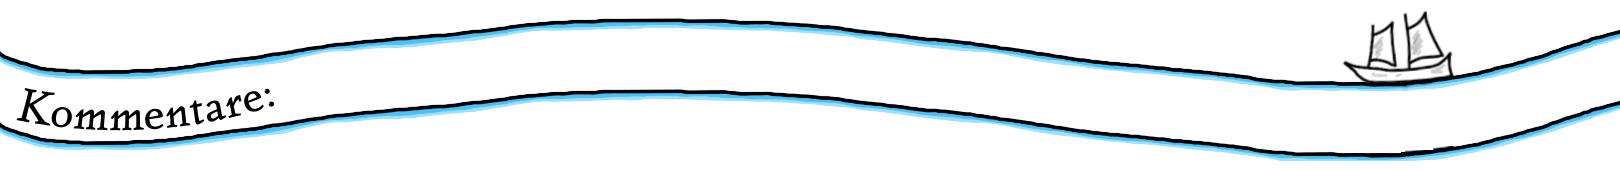
\includegraphics[keepaspectratio=true, width=\paperwidth]{mittelwelle.png}
		\fi
	\end{figure}
}
